\section{The upper bound}\label{sec:upper}

In this section $\beta=\beta(\alpha)<\infty$ and $\theta\in\Ga^*$ is fixed. For $c,\zeta>0$ let $n_G(\theta,c,\zeta)$ be an index such that $|\sin(2\pi q_n\theta)|\ge e^{-\zeta q_n}$ for all $n\ge n_G(\theta,c,\zeta)$ with $b_n\ge c$. The thresholds $n_0$ below may depend on $\theta$ through $n_G$, applied with parameters fixed before $n$ and $T$ vary, and the time threshold in Lemma~\ref{lem:covering} may depend on $\theta$ as well. The constants $C$ do not, since Proposition~\ref{prop:local} and Theorem~\ref{thm:window} are uniform over phases satisfying the sine condition at the scale used. All of these are fixed before $n$ and $T$ vary.

\subsection{Logarithmic windows at scales with a definite ratio}

\begin{proposition}\label{prop:selected}
Let $0<a<1$, $m>0$, $c>0$ and $0<d<B$, and let $B_0>\beta$ satisfy $f_0:=\max\{0,1-L/B_0\}<a$. There are $C$ and $n_0$ such that for every $n\ge n_0$ with $b_n\ge c$ and every $T$ with $e^{dq_n}\le T\le e^{Bq_n}$,
\[
P(T^a,T)\le CT^{-m}.
\]
\end{proposition}

\begin{proof}
Choose $\eta>0$ with $2\eta<ad/4$, then $\eps>0$ with $\eps<ad/4$ and $\eps/d<(a-f_0)/2$. Since $\limsup b_n=\beta<B_0$, we may take $n_0\ge\max\{n_G(\theta,c,\zeta_1),n_G(\theta,c,\eps_2)\}$, where $\zeta_1$ is given by Theorem~\ref{thm:window} for the parameters below and $\eps_2$ is defined in the second case, so large that $b_n\le B_0$ for $n\ge n_0$. Write $q=q_n$, $b=b_n$ and $\tau=\log T/q\in[d,B]$.

\emph{Case $b\ge L+2\eta$.} Apply Theorem~\ref{thm:window} with this $\eta$ and $\eps$, $\Lambda=\max(1,B)$ and $M=mB$. It gives $P(R_n(T),T)\le Ce^{-mBq}\le CT^{-m}$. Moreover
\[
\frac{\log R_n(T)}{\log T}\le\frac{\eps}{d}+\frac{\log2}{dq}+\frac{\max\{0,\min(\tau-L,\,b-L)\}}{\tau}.
\]
The last term is at most $1-L/b\le f_0$, since $b>L$. Indeed, it equals $0$ if $\tau\le L$, equals $1-L/\tau\le1-L/b$ if $L<\tau\le b$, and equals $(b-L)/\tau\le(b-L)/b$ if $\tau\ge b$. Hence $\log R_n(T)/\log T<(a+f_0)/2+o(1)<a$ for large $n$, so $R_n(T)\le T^a$ and $P(T^a,T)\le P(R_n(T),T)\le CT^{-m}$.

\emph{Case $c\le b<L+2\eta$.} Apply Proposition~\ref{prop:local} with $\eps_2=\min\{\eps/3,\min(L,c)/8\}$. Since $|\sin2\pi q\theta|\ge e^{-\eps_2q}$, its last assertion gives $N_n\le3e^{(2\eta+3\eps_2)q}\le T^a$ for large $q$, since $2\eta+3\eps_2<ad/4+ad/4=ad/2$ and $T\ge e^{dq}$. Hence
\[
P(T^a,T)\le P(N_n,T)\le C(1+e^{2Bq})\exp\bigl(-\eps_2e^{\eps_2q/2}/900\bigr)\le e^{-mBq}\le T^{-m}
\]
for large $q$. All parameters were fixed before $n$ and $T$ vary.
\end{proof}

When $\beta\le L$ one may take $B_0<L+2\eta$, and then only the second case occurs.

\subsection{Covering every time}

\begin{lemma}\label{lem:covering}
Let $a\in(0,1)$ with $a>\max\{0,1-L/\beta\}$ and let $m>0$. Then $P(T^a,T)=O(T^{-m})$ as $T\to\infty$.
\end{lemma}

\begin{proof}
Let $C_D,\kappa$ be as in Proposition~\ref{prop:dt}. Fix $K\ge1$ with $\kappa K>m+3$, and put $d=1/K$ and $c=a/(2K)$. Fix $B_0>\beta$ with $\max\{0,1-L/B_0\}<a$, and put $B=\max\{2B_0/a,2d\}$. Let $C$ and $n_0$ be given by Proposition~\ref{prop:selected} for these parameters and the fixed phase $\theta$.

For large $T$ let $j$ be the least index with $q_j\ge K\log T$. Two cases exhaust all possibilities.

\emph{Case A: $q_j\le T^a/(2C_D)$.} Let $N=\lfloor T^a\rfloor$, so $N\ge C_Dq_j$ for large $T$. Proposition~\ref{prop:dt} gives
\[
P(T^a,T)\le P(N,T)\le Ce^{-c_D(T^a-1)}+CT^3e^{-\kappa q_j}\le Ce^{-c_D(T^a-1)}+CT^{3-\kappa K}=O(T^{-m}).
\]
This case uses no information about the phase and allows arbitrarily long stretches of scales with small ratios.

\emph{Case B: $q_j>T^a/(2C_D)$.} Let $q=q_{j-1}$. By the choice of $j$, $q<K\log T$, so $\tau=\log T/q>d$. By~\eqref{eq:bn}, $q_j<D_{j-1}=e^{b_{j-1}q}$, so
\[
a\log T-\log(2C_D)<\log q_j<b_{j-1}q.
\]
Along a sequence of times in this case, $q_j\to\infty$, hence $j\to\infty$ and $q\to\infty$. Dividing by $q<K\log T$ gives $b_{j-1}>a/K-\log(2C_D)/q\ge a/(2K)=c$ for large $T$. Also $b_{j-1}\le B_0$ for large $j$, so $\tau<(B_0+\log(2C_D)/q)/a\le B$. Thus $T\in[e^{dq},e^{Bq}]$ and $b_{j-1}\ge c$. Since $\theta\in\Ga^*$ and $j-1\ge n_0$ for large $T$, Proposition~\ref{prop:selected} gives $P(T^a,T)\le CT^{-m}$.
\end{proof}

The covering needs no information about the scales between $q_{j-1}$ and $q_j$ other than the two inequalities above. In particular it allows $\liminf_n\beta_n=0$. Figure~\ref{fig:covering} shows how the two cases assign every large time to a single scale.

\begin{figure}[t]
\centering
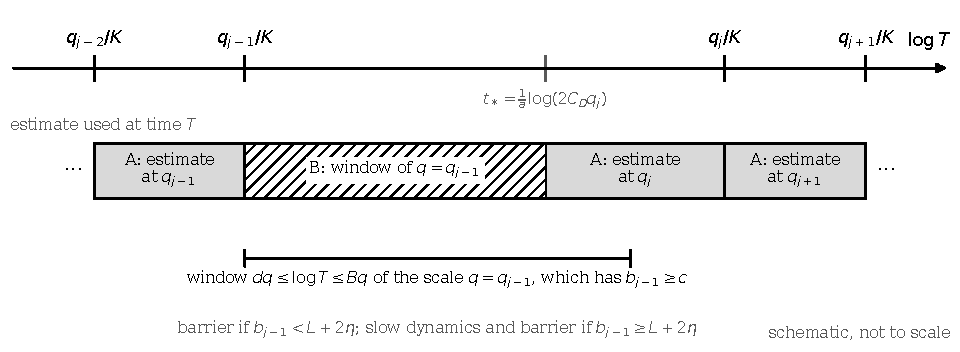
\includegraphics[width=\textwidth]{fig_covering.pdf}
\caption{Schematic of the time covering in the proof of Lemma~\ref{lem:covering}; not to scale, and the positions of the denominators are arbitrary. Here $\beta(\alpha)<\infty$ and $\theta\in G_\alpha^*$ is fixed. Fix $a\in(\max\{0,1-L/\beta(\alpha)\},1)$ and $m>0$, choose $K\ge1$ with $\kappa K>m+3$, and for a large time $T$ let $q_j$ be the first denominator with $q_j\ge K\log T$, so that $\log T\in(q_{j-1}/K,q_j/K]$. If $q_j\le T^a/(2C_D)$, that is, if $\log T\ge t_*$ (case~A, shaded), Proposition~\ref{prop:dt} at the scale $q_j$ gives $P(T^a,T)=O(T^{-m})$. Otherwise (case~B, hatched), which can happen only after a jump from $q_{j-1}$ to a denominator $q_j>e^{aq_{j-1}/K}/(2C_D)$, the scale $q=q_{j-1}$ has $b_{j-1}\ge c=a/(2K)$ and $\log T/q\in[d,B]$, where $d=1/K$, $B_0>\beta(\alpha)$ is chosen with $\max\{0,1-L/B_0\}<a$, and $B=\max\{2B_0/a,2d\}$. Proposition~\ref{prop:selected} then applies, through the barrier of Proposition~\ref{prop:local} or through Theorem~\ref{thm:window}, according as $b_{j-1}$ is below or at least $L+2\eta$, for the small $\eta>0$ fixed in its proof. Every sufficiently large time falls in one of the two cases, whatever the ratios $b_n$ at other scales; no regularity of these ratios and no overlap of windows at consecutive denominators is assumed.}
\label{fig:covering}
\end{figure}

\begin{theorem}\label{thm:upper}
Let $\lambda>1$, let $\alpha$ be irrational with $\beta(\alpha)<\infty$, and let $\theta\in\Ga^*$. For every $a>\max\{0,1-L/\beta(\alpha)\}$ and every $m>0$, $P(T^a,T)=O(T^{-m})$. Consequently
\[
\au(H_{\lambda,\alpha,\theta})\le\max\Bigl\{0,\ 1-\frac{\log\lambda}{\beta(\alpha)}\Bigr\}.
\]
\end{theorem}

\begin{proof}
For $a<1$ this is Lemma~\ref{lem:covering}. For $a\ge1$ choose $a'\in(\max\{0,1-L/\beta\},1)$ and use $P(T^a,T)\le P(T^{a'},T)$. The bound on $\au$ follows from Lemma~\ref{lem:moments}(3), letting $a$ decrease to $\max\{0,1-L/\beta\}$.
\end{proof}
